\section{Discussion}





\subsection{Nitrite Investigations}
We have found that  both disposable and reusable gold electrodes are suitable for measuring nitrite concentrations solutions from 0-96$\mu$M, reflecting the normal physiological serum levels and the expected elevation in septic patients (52.8$\pm$44.0 vs 29.6$\pm$8.9) \cite{pmid12688539}.Therefore, DPV is found to be a reliable method of measuring the electrochemical activity of nitrite in solution. However, using our parameters, each measurement takes 405s; This may prove a challenge for real-time monitoring and clinical settings.\\\\
DPV voltammograms from nitrite experimentation reveal a common peak where the peak current increases with higher concentrations of nitrite, across all experiments, between 0.7 and 0.8V, which is as expected from the literature \cite{article}. Small peaks corresponding to an unknown species were reliably detected at 0.2V in PBS only experiments but were not present in albumin experiments. Increased noise and smoothing may have eliminated this peak. We hypothesise that small peaks may have resulted from oxygen gas in the  solution.\\\\
The albumin experiments showed that at low nitrite concentrations (below 16 µM), the sensitivity is comparable to results without albumin. However, at higher nitrite concentrations, the sensitivity increases to 7nA/$\mu$M, with a marked change in the calibration curve (Figure 8), suggesting interactions between the nitrite and the albumin. The detected current was greater overall in albumin experiments compared to without albumin; This contradicts the hypothesis that albumin adsorbs onto the electrode surface, blocking mass transport and inhibiting electron transfer, interfering with the electrode's ability to detect nitrite.

\subsection{Hydrogen Peroxide Investigations}
In this study, a H$_{\text{2}}$O$_{\text{2}}$ calibration curve with gold electrodes was produced with concentrations from 0 to 300$\mu$M, which has ranged over the \textit{in-vivo} concentrations found in both healthy individuals the septic patients \cite{FORMAN201648, VanAsbeck1995}. Further, we validated the experimental concentrations by coulometry, finding that consistency was achieved between the experimental and theoretical concentrations.\\\\
It is observed that under low H$_{\text{2}}$O$_{\text{2}}$ concentrations (below 100$\mu$M), there are significant percentage differences between the experimental and theoretical concentration values (\autoref{tab:h2o2_col_res}). In the future, careful selection of the equipment for liquid transferring is critically required; Thus, an improvement of the experimental accuracy can be accomplished. Also, a non-linearity condition was observed in the current vs time plot under high H$_{\text{2}}$O$_{\text{2}}$ concentrations ($c>300$$\mu$M). By performing quantitative analysis based on \autoref{eqn:h2o2redox2} and the actual amount of reactants involved in the experiment, an approximation of the H$_{\text{2}}$O$_{\text{2}}$ concentration limit was found to be at 280$\mu$M, indicating excess H$_{\text{2}}$O$_{\text{2}}$ concentration would result in insufficient PB for reaction with H$_{\text{2}}$O$_{\text{2}}$. 


\subsection{Lactate Investigations}
The differences in the current-concentration relationship conveyed in \autoref{fig:lactate_result}(b) and (c) can be explained by lactate oxidase enzyme kinetics.\\\\
The linear range is shown to be at 0.0-2.0mM lactate. The current detected is approximately entirely dependent on the lactate concentration. The electron flow is indicative of the reaction rate. 
%In this region of the graph, purely dependent on lactate concentration
% enzyme concentration or enzyme ability to allow binding has no effect on the sensing abilities.
After 2.0mM, the reaction rate can be seen as starting to plateau. Whilst there is no limit in detection observed in the concentration range tested, it can be assumed that it is being approached. Therefore, the relationship's non-linear behaviour is due to enzyme kinetics.\\\\
\begin{figure}[H]
    \centering
    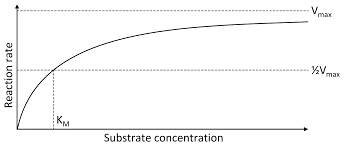
\includegraphics{img/lactate_discussion_1.png}
    \caption{Michaelis-Menten Kinetic plot of enzyme substrate reactions. }
    \label{fig:lactate_discussion}
\end{figure}
\noindent Michaelis-Menten equations for reaction velocity \cite{johnson2011original}:
\begin{equation}
    E + S \xrightleftharpoons[k_{\text{off}}]{k_{\text{on}}} ES \xrightarrow{k_{cat}} E+P \quad \quad v = \frac{V_{max}[S]}{K_{M}+[S]}
\end{equation}
Enzyme kinetics can be defined partially by their Michaelis constant, $K_{m}$, which describes the lactate concentration at which the current is half the maximum current at the detection limit seen in \autoref{fig:lactate_discussion}. In the Michaelis- Menten model, $v$ represents reaction velocity. We can take current to be proportional to $k_{cat}$ and, hence, proportional to the velocity of the H\textsubscript{2}O\textsubscript{2} production. From the Michaelis-Menten equation, as $V_{max}$ and Km are constants, the plot is hyperbolic, and at higher concentrations, we can expect a decreased climb in velocity; Our calibration plot is in accordance with this. Since Michaelis-Menten kinetic models require that the LOX immobilisation in the matrix does not affect its affinity for lactate, we instead approximate a value for $K_{m}$ by calculating an apparent constant $K_{m[app]}$.  Based on our calibration curve, we can approximate $v_{max}$ to be $4.04\times10^{-6}$A; This gives a $K_{m[app]}$ proportional to the concentration where a current of $2.02\times 10\textsuperscript{-6}$A would be observed at approximately 1.0mM.\\\\
We can conclude that the Nafion membrane modified sensor is useful for detecting concentrations in the range experimented. As the same clinical course of action is taken for patients exhibiting lactate levels above 3.5mM, the plateau in reading in the upper range of lactate concentrations is not a significant issue for diagnosing sepsis. A Levich study of these lactate sensors would allow us to define parameters regarding mass transport and kinetics around the RDE, allowing us to compare detection with different modifications to electrode design \autoref{app:Lactate_future}.
\subsection{Aptamer Modelling}
In this study, we have developed a novel NIL algorithm capable of decomposing multi-exponential chronoamperometric current signals. We showed that this algorithm is able to resolve rate constants up to a resolution of $k_{A} = 200s^{-1}$ and $k_{AT} = 400s^{-1}$, on simulated signals with realistic noise levels. Accurate estimates were also obtained for the coefficients, showing the algorithm's accuracy in obtaining the target concentration, [T]. These rate constants values are closer compared to the $k_{A} = 125s^{-1}$ and $k_{AT} = 500s^{-1}$ quoted in Plaxco's study \cite{arroyo2018subsecond}.\\\\
In parallel, we develop a coarse-grained model of aptamers by assuming it as a freely-jointed chain to gain insight into the physical effects of target binding. We generate length probability distributions and assess how the probability of a collision event $P(L<1.5\text{nm})$ varies with aptamer length. These estimates correlate with aptamer modelling studies in the literature \cite{uzawa2010mechanistic,uzawa2009length}.